
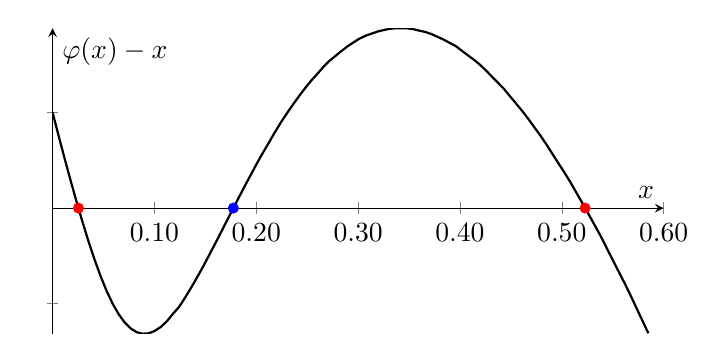
\begin{tikzpicture}[scale=1.0]

\begin{axis}
[
  title={},
  width  = 0.8*0.8*\columnwidth,
  height = 0.8*0.4*\columnwidth,
  axis lines=center,
  legend style={at={(0.95,0.95)}, anchor=north east},
%   xmode=log,
  xlabel={$x$},
  ylabel={$\varphi(x)-x$}, ylabel style={rotate=0},
%  yticklabel=\pgfmathprintnumber{\tick}\\ \%,
  xmin = 0.0, 	
  xmax = 0.6,
%   ymin = -0.05,
%   ymax = 0.05,
  scaled y ticks = false,
  yticklabels={,,},
%   y tick label style={
%         /pgf/number format/.cd,
%         fixed,
%         fixed zerofill,
%         precision=2,
%         /tikz/.cd
%   },
  x tick label style={
        /pgf/number format/.cd,
        fixed,
        fixed zerofill,
        precision=2,
        /tikz/.cd
  },
%   grid = both,
  scale only axis,
]
	\legend{}
    
    \def\k{0.012}
    \def\p{0.100}
    \foreach \a in {0.002}
        \addplot[thick, domain = 0:0.585, samples=100] {(\k*(\a/\p)-\p*x*(\a/\p)^(\k/(\p*x)))/(\k-\p*x)-x};
    
    \fill[color = red]  (axis cs: 0.02539, 0) circle[radius=2pt];
    \fill[color = blue] (axis cs: 0.17750, 0) circle[radius=2pt];
    \fill[color = red]  (axis cs: 0.52286, 0) circle[radius=2pt];
    
    % \foreach \a in {0.1,0.2,0.3,0.4,0.5,0.555,0.62}
    %     \addplot[domain = 0:1, samples=100] {(k*(a/p)-p*x*(a/p)^(k/(p*x)))/(k-p*x)-x};
    
    % \addplot[domain = 0.5:1.04, dashed, samples=100] {x*(1+((-3 + 2*x + sqrt(5 + 4*(-1 + x)*x))/(2*x))*x)*exp(-(2-((-3 + 2*x + sqrt(5 + 4*(-1 + x)*x))/(2*x)))*x)};
    
%     \addplot[thick] table
%     [
% 		x expr = \thisrow{lam},
%     	y expr = \thisrow{25dB}
%     ] {./Data/envelopes.dat};

    % \draw[-\arrowhead] (axis cs: 0.8,0.08) -- (axis cs: 2.7,0.27) node[anchor=south west] 
    %     {$\alpha = 0.1,0.2,0.3,0.4,0.5,0.56,0.62$};
\end{axis}

\end{tikzpicture}
